\documentclass{beamer}
\usetheme{metropolis}
\usepackage{graphicx}
\usepackage{tcolorbox}
\title{Safe Return Doubtful: Week 9}
\date{\today}
\author{Jordan Hanson}
\institute{Whittier College Department of Physics and Astronomy}

\begin{document}
\maketitle

\section{Summary}

\begin{frame}{Summary}
\textbf{Climate science}
\begin{enumerate}
\item \textbf{How do we know} adding ice to ocean will cause sea level rise? (The ice cubes in a glass concept).
\item How do we know \textbf{historical} temperature of ice?
\item How do we know the speed of ice flowing into ocean?
\end{enumerate}
\end{frame}

\section{Adding Ice to Ocean and Sea Level Rise}

\begin{frame}{Antarctic Ice and the Ocean - Examples}
The density of something is the mass divided by the volume:
\begin{equation}
\rho = \frac{m}{V}
\end{equation}
The units can be kilograms per meter cubed, or kg/m$^{3}$.  If we know the density of a material and the volume, we can know the mass of the object:
\begin{equation}
m = \rho V
\end{equation}
(Examples).
\end{frame}

\begin{frame}{Antarctic Ice and the Ocean - Examples}
The force of gravity, or weight (as we saw once before) is the mass of an object, times the gravitational \textit{acceleration}, called $g$:
\begin{equation}
w = mg
\end{equation}
The value of $g$ is 9.81 meters per second squared, or 9.81 m/s$^2$.  When an object floats, the buoyant force must balance the weight. When a mass in kilograms is multiplied by $g$, the units of force are \textit{Newtons.}  (Examples).
\end{frame}

\begin{frame}{Antarctic Ice and the Ocean - Examples}
\begin{tcolorbox}[colback=white,colframe=red!40!blue,title=The buoyant force]
\alert{The buoyant force is an upward force placed on an object suspended in a liquid that is equal in magnitude to the weight force of the displaced volume of liquid.}
\end{tcolorbox}
Example, suppose a sailboat displaces 45 cubic meters of water.  The weight force is equal to the mass of that water in the \textit{upwards direction.}  What's the mass of that water?  $m = \rho V$, so $m = 1000$ kg/m$^3 \times 45$ m$^3$, so 45,000 kg.  What is the \textit{weight} of that water?  $w = mg$, so $w = 45,000$ kg $\times 9.81$ m/s$^2$, or 441,450 Newtons (about 99,000 lbs).
\end{frame}

\begin{frame}{Antarctic Ice and the Ocean - Examples}
What is the \textit{weight} of that water?  $w = mg$, so $w = 45,000$ kg $\times 9.81$ m/s$^2$, or 441,450 Newtons (about 99,000 lbs).
\begin{figure}
\centering
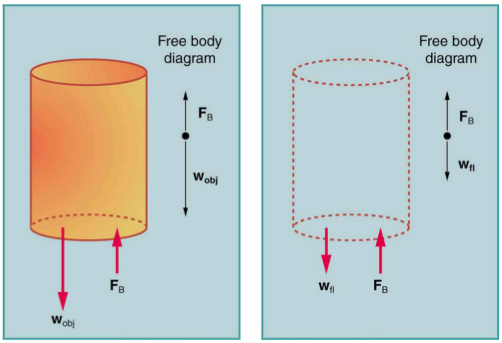
\includegraphics[width=0.6\textwidth]{buoy.png}
\caption{\label{fig:buoy} A diagram of the buoyant force balancing the weight.}
\end{figure}
\end{frame}

\begin{frame}{Antarctic Ice and the Ocean - Examples}
\textbf{Questions for table discussion:}
\begin{itemize}
\item Given what you've seen, why does a ship made of metal float?  Isn't metal more dense than water?
\item What is the weight force in Newtons of a person with mass 55 kg?
\item What is the weight of an ice cube that is a cube of 10 cm on each side, and the density of ice is 918 kg/m$^3$?
\end{itemize}
\end{frame}

\begin{frame}{Antarctic Ice and the Ocean - Examples}
\textbf{Questions for table discussion:}
\begin{itemize}
\item Given what you've seen, why does a ship made of metal float?  Isn't metal more dense than water?
\item What is the weight force in Newtons of a person with mass 55 kg?
\item What is the weight of an ice cube that is a cube of 10 cm on each side, and the density of ice is 917 kg/m$^3$?
\end{itemize}
\end{frame}

\begin{frame}{Antarctic Ice and Ocean Level Rise}
\begin{figure}
\centering
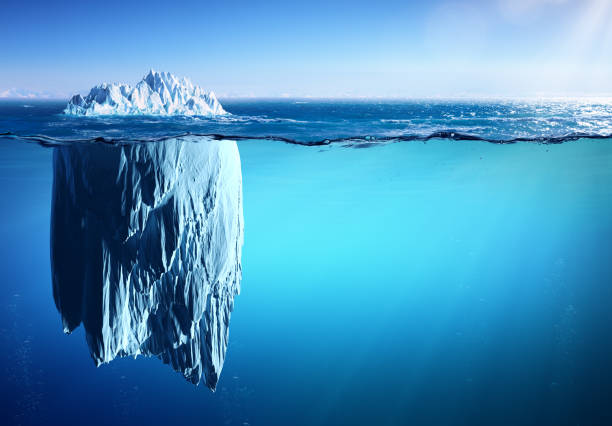
\includegraphics[width=0.7\textwidth]{ice.jpg}
\caption{\label{fig:ice} An iceberg is mostly below the water.  Can we determine what fraction of the iceberg is below the water, and therefore the displaced water?}
\end{figure}
\end{frame}

\begin{frame}{Antarctic Ice and Ocean Level Rise}
Suppose a block of ice of height $V$ and horizontal area $A$ is floating in the ocean.  The volume is
\begin{equation}
V = Ah
\end{equation}
Let the density of ice be $\rho_{\rm ice}$, and let the density of water be $\rho_{\rm w}$.  The weight of the iceberg is
\begin{align}
w &= mg \\
w &= \rho_{\rm ice} V g \\
w &= \rho_{\rm ice} A h g
\end{align}
\textbf{Table discussion:} What is the \textit{weight} of an iceberg that has an area of 1 km by 1 km on top, a height of 1 km?
\end{frame}

\begin{frame}{Antarctic Ice and Ocean Level Rise}
\small
Continuing, the weight of the iceberg is
\begin{equation}
w_i = \rho_{\rm ice} A h g
\end{equation}
How much water does the iceberg displace?  Let the height \textit{above} the water be $x_1$ and the depth below the water be $x_2$, such that $x_1 + x_2 = h$.  The displaced water volume is
\begin{equation}
V_d = A x_2
\end{equation}
The displaced water mass is $m_w = \rho_{w} V_d$, so
\begin{equation}
m_w = \rho_{w} A x_2
\end{equation}
The weight of the displaced water just requires us to multiply by $g$, so
\begin{equation}
W_w = \rho_{w} A x_2 g
\end{equation}
\end{frame}

\begin{frame}{Antarctic Ice and Ocean Level Rise}
Thus, we have the weight of the displaced water, $\rho_{w} A x_2 g$, and the weight of the iceberg, $\rho_{\rm ice} A h g$. According to the buoyant force principle, these two weights are \textbf{equal.}  Thus, 
\begin{equation}
\rho_{w} A x_2 g = \rho_{\rm ice} A h g
\end{equation}
Given that $h = x_1 + x_2$, let's simplify this...(board).
\begin{equation}
\frac{x_1}{x_2} = \frac{\rho_{\rm w} - \rho_{\rm ice}}{\rho_{\rm ice}} \label{eq:ice1}
\end{equation}
Equation \ref{eq:ice1} is the fraction of the iceberg that peaks above the surface.
\end{frame}

\begin{frame}{Antarctic Ice and Ocean Level Rise}
\begin{equation}
\frac{x_1}{x_2} = \frac{\rho_{\rm w} - \rho_{\rm ice}}{\rho_{\rm ice}} \label{eq:ice2}
\end{equation}
Equation \ref{eq:ice2} is the fraction of the iceberg that peaks above the surface.  Given that you can see $\approx 10$ percent of an iceberg, and that $90$ percent is beneath the surface, we know how much water is displaced. \\
\begin{equation}
V_{wd} = A x_1 \left(\frac{\rho_{\rm ice}}{\rho_{\rm w} - \rho_{\rm ice}}\right)
\end{equation}
What is the water level rise if we toss an iceberg into a giant bucket of water? \\ \vspace{0.5cm}
Suppose the giant bucket has a length and a width of $l$, so an area of $l^2$.  What is the water level rise $\Delta y$?
\end{frame}

\begin{frame}{Antarctic Ice and Ocean Level Rise}
Here's how to solve for it:
\begin{align}
l \times l \times \Delta y &= V_{wd} \\
\Delta y &= \frac{Ah}{l^2}\left(\frac{\rho_{\rm ice}}{\rho_{\rm w}}\right)
\end{align}
What is the sea level rise if $l = 1$ km, $h = 1$ km, and $A = 1$ km$^2$?  Recall that ice density is 917 kg/m$^3$, and water density is 1000 kg/m$^3$.
\end{frame}

\begin{frame}{Antarctic Ice and Ocean Level Rise}
So that was an example of how adding ice to the ocean causes sea level rise.  Here is a short video summary of research into Antarctic and Greenland contributions to sea level rise: \\ 
\url{https://youtu.be/YRe1ymYR45k} \\ \vspace{1cm}
And here is how certain people view the science: \\
\url{https://youtu.be/lPgZfhnCAdI}
\end{frame}

\section{Historical Data from Ice Cores}

\begin{frame}{Historical Data from Ice Cores}
\small
\begin{figure}
\centering
\includegraphics[width=0.75\textwidth]{bubbles2.jpg}
\caption{\label{fig:bubbles2} A sliver of Antarctic ice showing hundreds of tiny trapped air bubbles.  Air bubbles trapped in ice hundreds or even thousands of years ago are providing vital information about past levels of greenhouse gases in the Earth's atmosphere.}
\end{figure}
\end{frame}

\begin{frame}{Historical Data from Ice Cores}
\small
\begin{figure}
\centering
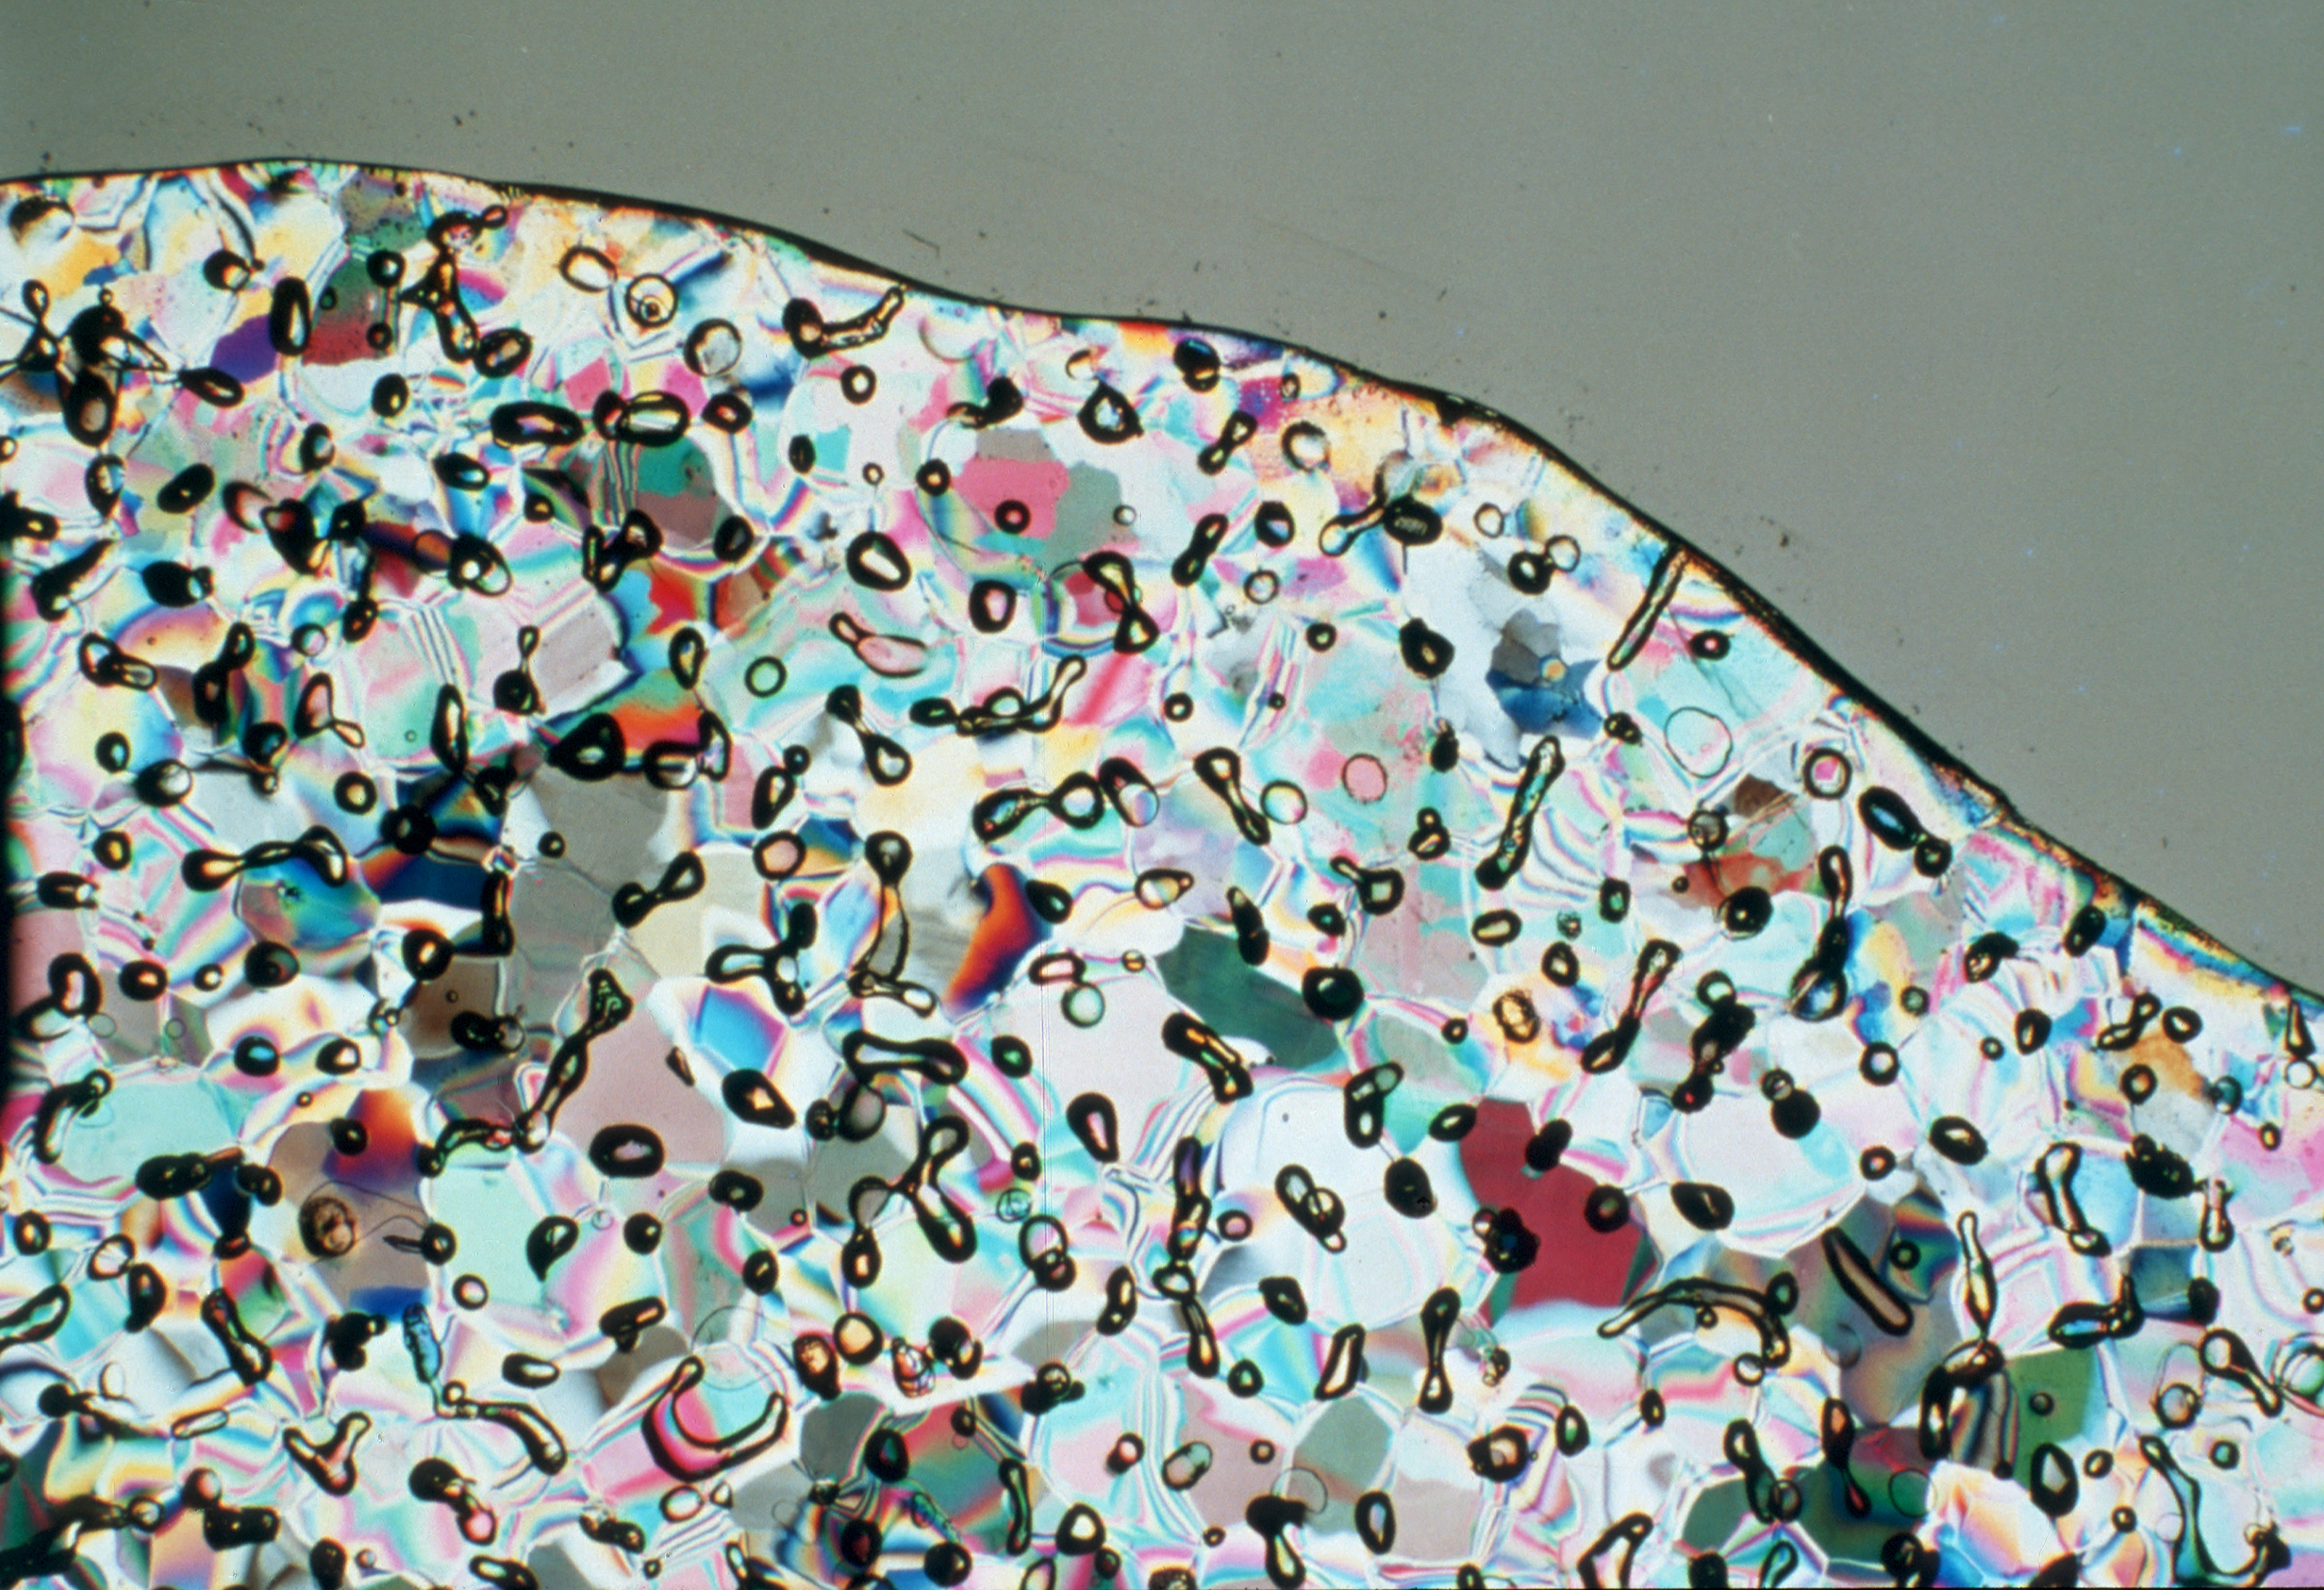
\includegraphics[width=0.75\textwidth]{bubbles.jpg}
\caption{\label{fig:bubbles} A sliver of Antarctic ice showing hundreds of tiny trapped air bubbles.  Polarized light reveals more of the crystal structure.}
\end{figure}
\end{frame}

\begin{frame}{Historical Data from Ice Cores}
Air bubbles are trapped as the ice forms, and then saved beneath the surface as they are transported downwards for thousands of years.
\begin{itemize}
\item \textbf{Light-colored layers}: from snow accumulation during the summer when there is fresh precipitation.
\item \textbf{Dark-colored layers}: from dust and snow moved around by wind during winter when there is relatively less fresh snow.
\end{itemize}
\textit{Like counting tree-rings, we can measure the age of an ice layer in years ``before present'' (BP).}
\end{frame}

\begin{frame}{Historical Data from Ice Cores}
Air bubbles are trapped as the ice forms, and then saved beneath the surface as they are transported downwards for thousands of years.
\begin{itemize}
\item \textbf{Isotope}: a type of atom having different number of neutrons in the nucleus.  Example: Oxygen-18, Deuterium (D)
\item \textbf{Isotope variation}: Ancient air in ice cores shows seasonal variation of $O_{18}$ vs. $O_{16}$ and $H$ vs. $D$  The heavier isotopes are preferentially left behind when evaporation occurs, and liquid water transport occurs.  This is known as \textit{fractionation.}
\end{itemize}
\end{frame}

\begin{frame}{Historical Data from Ice Cores}
After subtracting seasonal variations, scientists look at the fractional deficit of Oxygen-18 or Deuterium:
\begin{equation}
\delta O18 = \frac{O18-O16}{O16} \times 100.0
\end{equation}
\begin{itemize}
\item $\delta O18$/$\delta D$: larger deficits indicate higher temperatures
\item The oxygen and hydrogen originally come from $H_2 O$.
\end{itemize}
\end{frame}

\begin{frame}{Historical Data from Ice Cores}
After subtracting seasonal variations, scientists look at the fractional deficit of Oxygen-18 or Deuterium:
\begin{figure}
\centering
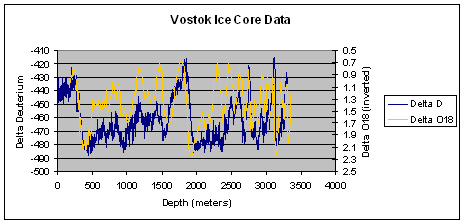
\includegraphics[width=0.75\textwidth]{Vostok_deltaD_deltaO18.jpg}
\caption{\label{fig:vostok} Changes in $dO18$ and $dD$ track changes in climate.  Ice ages can be revealed, for example.}
\end{figure}
\end{frame}

\begin{frame}{Historical Data from Ice Cores}
After subtracting seasonal variations, scientists look at the fractional deficit of Oxygen-18 or Deuterium:
\begin{figure}
\centering
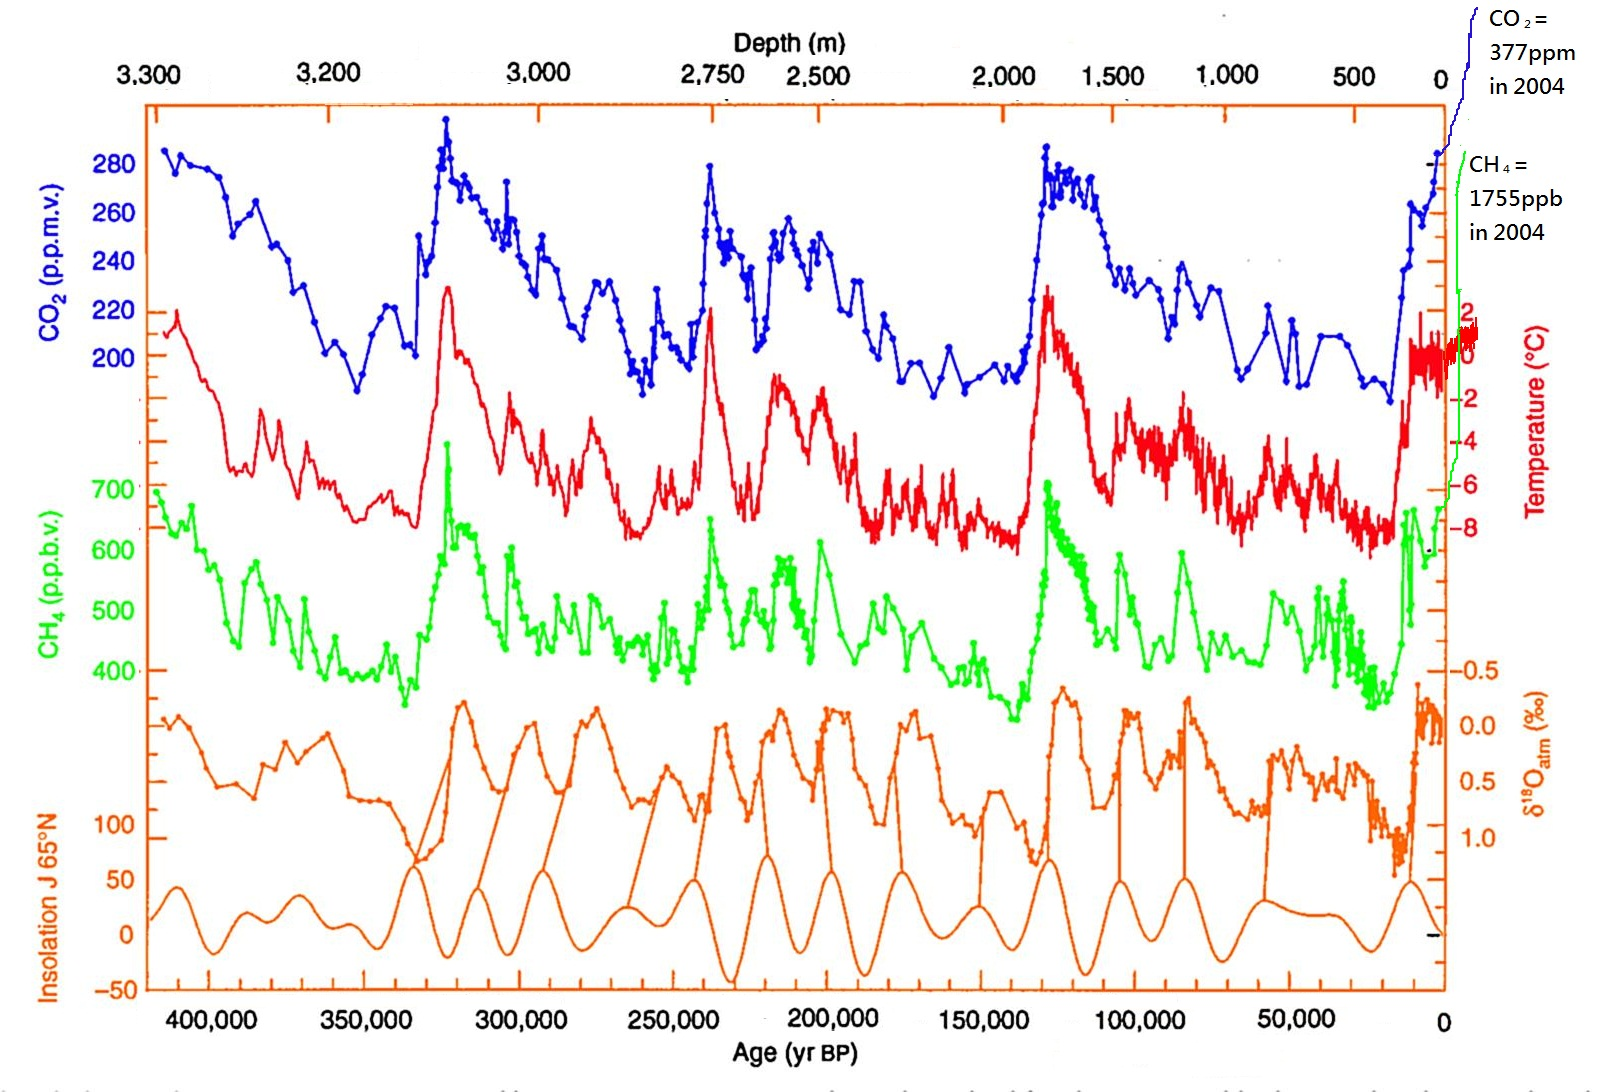
\includegraphics[width=0.7\textwidth]{Vostok2.jpg}
\caption{\label{fig:vostok2} Changes in $dO18$ and $dD$ track changes in climate.  Connection to temperature has to be calibrated.}
\end{figure}
\end{frame}

\section{Activity: Obtaining and Graphing Ice Core Data from NOAA}

\begin{frame}{Historical Data from Ice Cores}
Follow this link to the NOAA database for ice core data: \\
\url{https://www.ncdc.noaa.gov/data-access/paleoclimatology-data/datasets/ice-core}
\begin{enumerate}
\item Click on interactive map.
\item Click on base maps in the upper right hand corner and select countries.
\item Use the Paleo network tools: rectangle to select the South Pole as a site.  How do you know which ice core site is the South Pole?
\item After finding the South Pole site, click on the EPICA data set at left: access data.
\item Scroll down and download the text file ``edml-co2-2005.txt''
\end{enumerate}
\end{frame}

\begin{frame}{Historical Data from Ice Cores}
Follow this link to the NOAA database for ice core data: \\
\url{https://www.ncdc.noaa.gov/data-access/paleoclimatology-data/datasets/ice-core}
\begin{enumerate}
\item In the file, find the data by scrolling down.  You can view the data in Excel, but it should be presented in HTML first by clicking on it.
\item Copy the data into Excel and graph carbon dioxide in ppmv (parts per million by volume) versus gas age (year AD).
\item What do you observe about the carbon dioxide concentration?
\end{enumerate}
\end{frame}

\begin{frame}{Summary}
\textbf{Climate science}
\begin{enumerate}
\item \textbf{How do we know} adding ice to ocean will cause sea level rise? (The ice cubes in a glass concept).
\item (Next time): How do we know \textbf{historical} temperature of ice?
\item (Next time): How do we know the speed of ice flowing into ocean?
\end{enumerate}
\end{frame}

\end{document}